\subsection{Results} \label{subsec:results_logistic_regression}
Using scikit's grid search functionality it can be shown that both a rbf and a linear kernel with $C=1$ are a good choice for the support vector machine. Therefore, we will use a linear kernel and set $C=1$. 

\begin{table}[H]
\begin{tabular}{@{}lllll@{}}
\toprule
Classification Method                   & TP (train) & TN (train)   & TP (test)   & TN (test)   \\ \midrule
logistic sgd                            & 0.94      & 0.99 & 0.90 & 0.97 \\
logistic sgd cv                         & 0.95      & 0.98 & 0.93 & 0.99 \\
logistic scikit                         & 0.94      & 0.99 & 0.90 & 1    \\
logistic scikit cv                      & 0.92      & 0.99 & 0.90 & 1    \\
svm                                     & 0.96      & 1    & 0.94 & 0.97 \\
svm cv                                  & 0.96      & 1    & 0.93 & 1   \\ \bottomrule
\end{tabular}
\caption{Performance of each classification method in terms of the true positive (TP) and true negative (TN) percentage for training and test data. We use the following hyperparameters: $\lambda=0.001$, learn rate=0.001, batchsize=1, epoch=1000, test ratio=0.1, k-fold=5.}  
\label{table:1}
\end{table}


From table \ref{table:1} it shows that SVM is the best performing classification algorithm. SVM is known to be capable of separating overlapping class distribution \cite{bishop2006pattern}. Logistic regression, on the other hand, requires too many hyperparameters that finding the best set of hyperparameters is another task aside from optimizing the learnable parameters. We can say that all methods perform well in classifying benign classes and perform average on classifying cancer, i.e. malignant tumors. 


\begin{figure}[H]
    \centering
    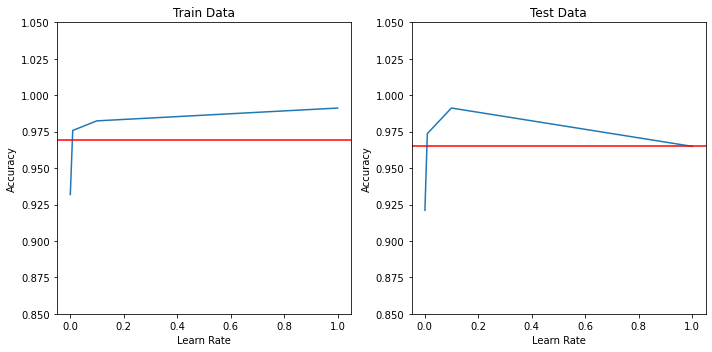
\includegraphics[width=1\linewidth]{Images/epoch100.png}
    \caption{Accuracy variation as a function of the learning rate for the case with the following hyperparameter: $\lambda=0.001$, batch size=32, epoch=100, test ratio=0.2}
    \label{fig:epoch100}
\end{figure}

To study the effect of tuning parameters in the performance of the model we examine the following cases: effect of the number of epoch and effect of the number of batches. 

In figure \ref{fig:epoch100} we see that the model starts to overfit as the learning rate increases, it is evident in the result of the testing accuracy. It is a result of a small number of iteration. One can improve the model by increasing the number of iterations, as seen in \ref{fig:epoch1000}, which starts performing well as a function of the learning rate.


\begin{figure}[H]
    \centering
    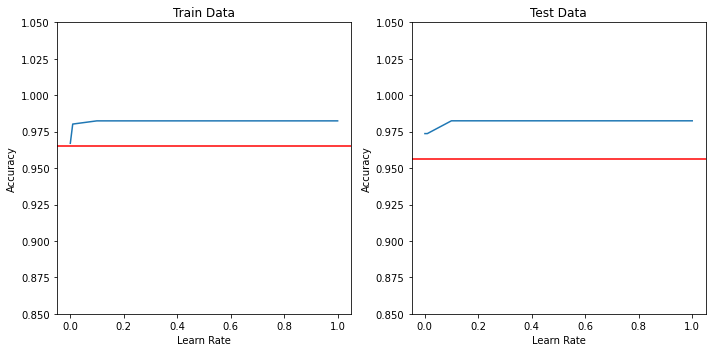
\includegraphics[width=1\linewidth]{Images/epoch1000.png}
    \caption{Accuracy variation as a function of the learning rate for the case with the following hyperparameter: $\lambda=0.001$, batch size=32, epoch=1000, test ratio=0.2}
    \label{fig:epoch1000}
\end{figure}

We explore also the effect of mini-batches size. The number of mini-batches determines the speed of the gradient search and thus helps minimize the chances of being stuck in a local minimum. This can be seen in figure \ref{fig:MS1}-\ref{fig:MS32} in both mini-batch cases. At standard stochastic gradient descent case (batch size=1) the accuracy increase is slow, as shown in the test accuracy of figure \ref{fig:MS1}, compared that to the second case where the mini-batch size is 32 shown in the test accuracy of figure \ref{fig:MS32}, the change of accuracy improves drastically. Basically, the batch size affects how quickly the model optimizes the learnable parameters. 



\begin{figure}[H]
    \centering
    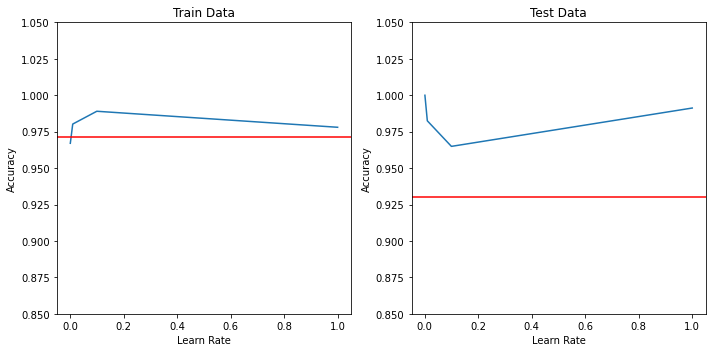
\includegraphics[width=1\linewidth]{Images/MS1.png}
    \caption{Accuracy variation as a function of the learning rate for the case with the following hyperparameter: $\lambda=0.001$, batch size=1, epoch=1000, test ratio=0.2}
    \label{fig:MS1}
\end{figure}

\begin{figure}[H]
    \centering
    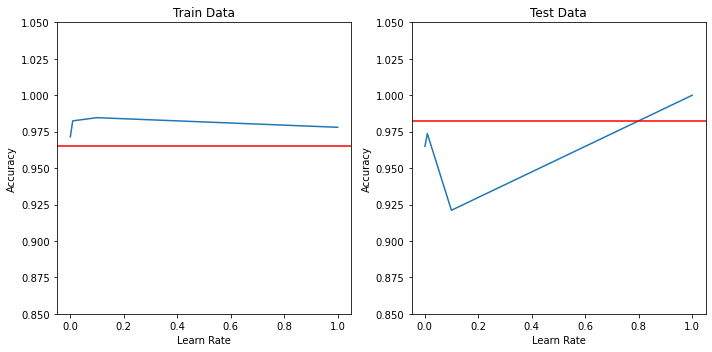
\includegraphics[width=1\linewidth]{Images/MS32.png}
    \caption{Accuracy variation as a function of the learning rate for the case with the following hyperparameter: $\lambda=0.001$, batch size=32, epoch=1000, test ratio=0.2}
    \label{fig:MS32}
\end{figure}